\section{Scaling Performance of $512^3$ problem}
Let us proceed now showing the performances achieved by our code in a large sized problem.
The present simulation shown a better scaling effectiveness and efficiency for both methods with respect to $128^{3}$ problem. 
\par
The best results are reached using 8 cores per processor, indicating that the efficiency lack cost overcome the message passing price.
In theory we would rather use a pure MPI approach instead of a heavily threaded ones, because the speedup achieved by the first method are significantly faster than the latter ones. However, for costing reasons, a tradeoff between the two solutions is preferred. \\
\par
The speedup peak is remarkable, with a factor above $480$ on $2048$ cores using pencil decomposition, while stops around $50$ using $128$ cores and slab decomposition. \\
\par

\begin{figure}
\begin{center}
\includegraphics[scale=0.6]{grafici/5121}
\caption{Scaling performance of $512^3$ simulation}
\label{5121}
\end{center}
\end{figure}

\begin{figure}
\begin{center}
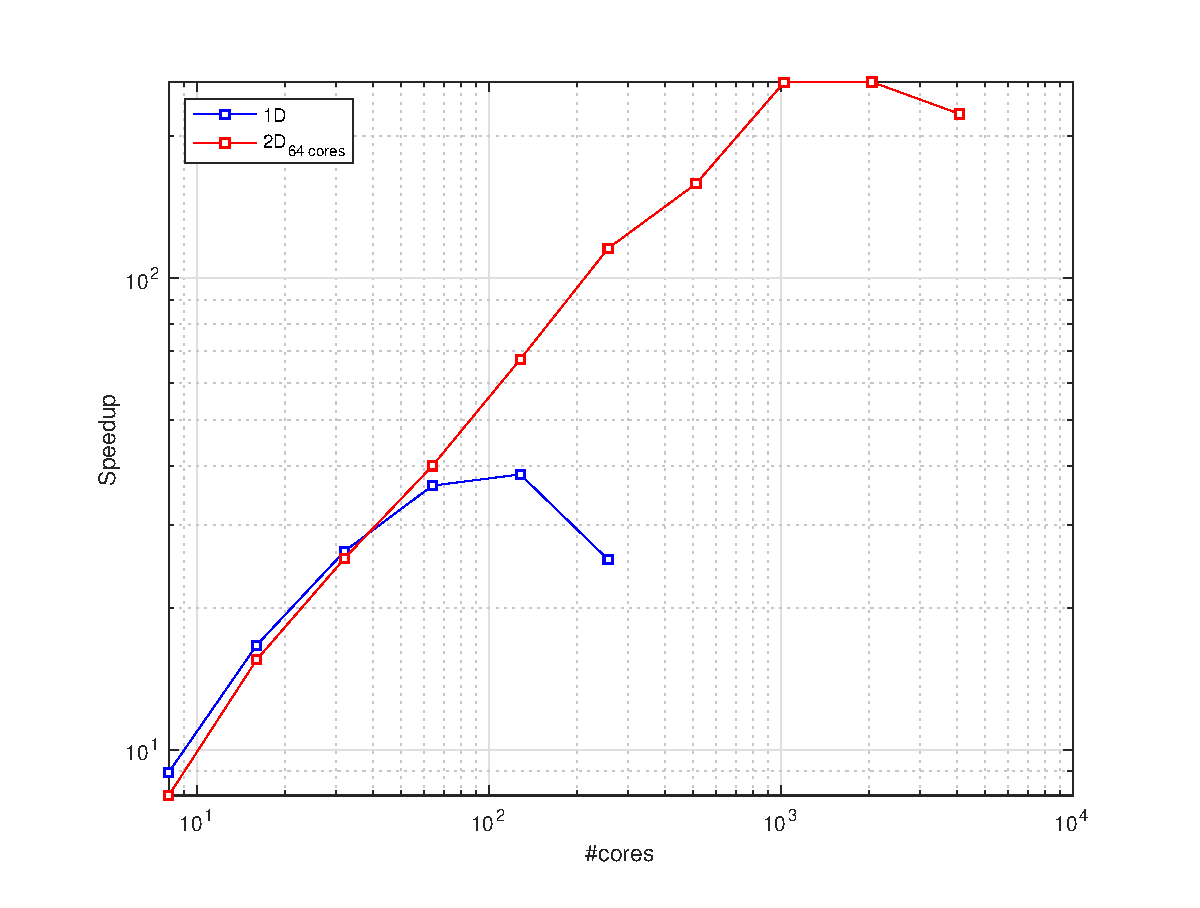
\includegraphics[scale=0.6]{grafici/5122}
\caption{Speedup factor of $512^3$ simulation}
\label{5122}
\end{center}
\end{figure}

As we can see from figure~\ref{5122}, where is compared the slab decomposition against the pencil ones running on 64 cores per processor, the speedup factor of the latter algorithm increase approximately linearly until $512$ cores. The raise in performance continue at lower factor until $2048$ cores are reached, where performances start decreasing. For what concern the first algorithm we face a sub-optimal linear increase in performances until 64 cores are reached. 
The inverse behaviors are shown in figure~\ref{5121}, where the simulation time is plotted against the number of processes.
\par
We refer to figure~\ref{5123} of page~\pageref{5123} to have an idea of the efficiency of the 1D decomposed algorithm. The figure shows that the efficiency remains near the $80\%$ until $32$ cores are used. However, once passed such limit, the behavior is still linear and smoother with respect to the ones shown in figure~\ref{644} of page~\pageref{644}.  \\
\par
It is interesting to denote how advantageous the 2D decomposed algorithm is; it is clear by looking at the figure~\ref{5121}. The time saving could be in the order of magnitude of $\mathcal{O}(10)$.\\
\par
It is evident that the pencil decomposition outclass the slab ones. However we could improve our results by selecting the proper number of threads per processor. 
---FINO A QUI---
\par
To decide what is the best solution we must evaluate the performances in an homogeneous way.
By looking at the values in table~\ref{512data:multi} of page~\pageref{512data:multi} and the depicted counter part, in figures~\ref{512:perf} and \ref{512:times}, it is possible to denote that between $16$ and $32$ cores, using 8 threads per processor, the behavior fits the ideal ones,  with really  small loss. This lead us to expect a perfect theoretical linear behavior spacing from $1$ to $32$ parallel tasks. Keeping this in mind, we feel confident and seems reasonable to consider a speedup factor of $16$ for the $16$ processes simulation using 8 cores, possibly making a small error. According to this we will take the performances of this point as reference.\\
\par


\begin{figure}
\begin{center}
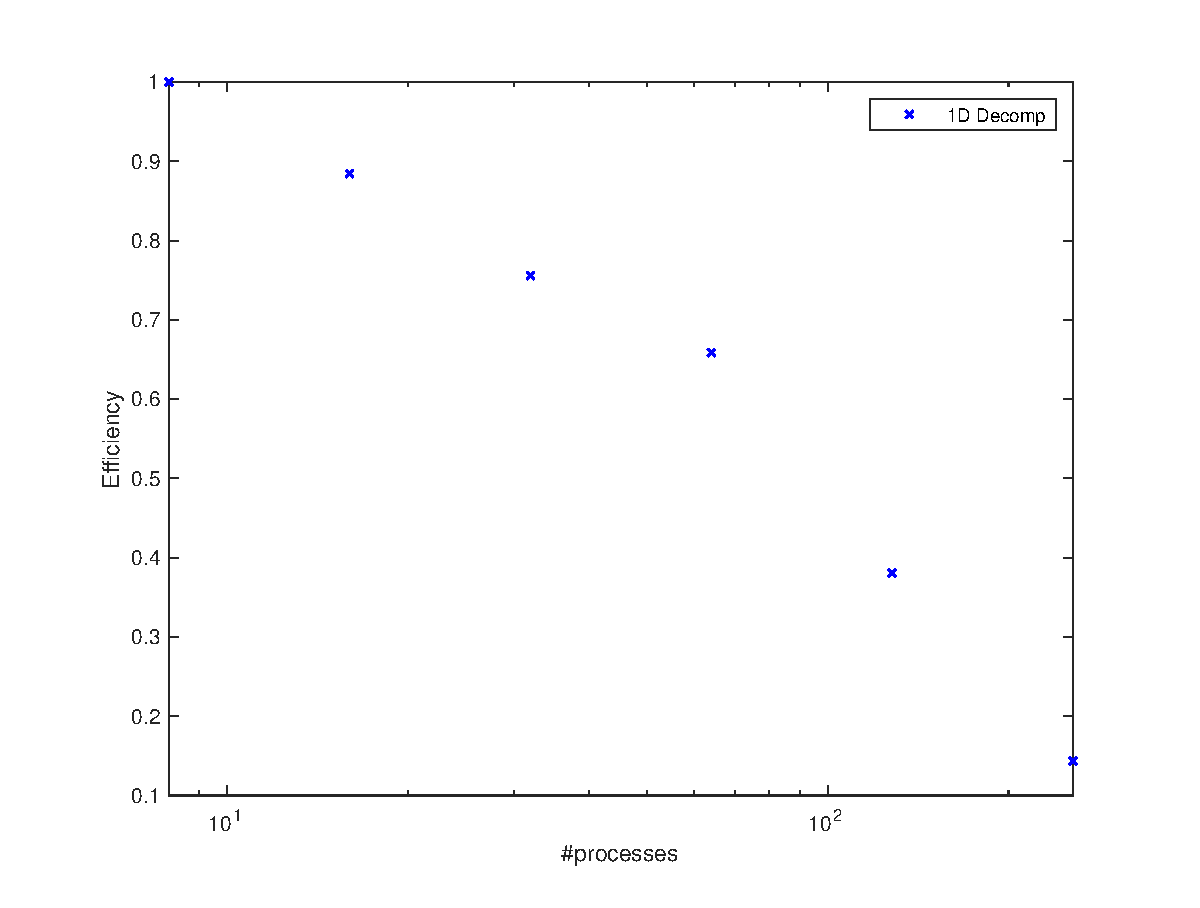
\includegraphics[scale=0.6]{grafici/5123}
\caption{Efficiency factor of $512^3$ simulation}
\label{5123}
\end{center}
\end{figure}

\begin{table}[h]
\caption{Data from $512^{3}$ simulation}
\begin{center}
\begin{tabular}{c c c c c}
\toprule
\textbf{\#cores} & \textbf{Time [s]} & \textbf{Speedup} & \textbf{Efficiency [\%]} & \textbf{Decomp}\\
\midrule
\multirow{2}{*}{8} & 1750 & 8.96 & 100 &1D\\
& 1960 & 1 & 100 & 2D\\
\hline
\multirow{2}{*}{16} & 941.5 & 16.65 & 93 & 1D\\
& 1011 & 15.51 & 97 & 2D\\
\hline
\multirow{2}{*}{32} & 595.3 & 26.35 & 74 & 1D\\
& 616.2 & 25.45 & 80 & 2D\\
\hline
\multirow{2}{*}{64} & 432.1 & 36.3 & 51 & 1D\\
& 392.3 & 39.97 & 62 & 2D\\
\hline
\multirow{2}{*}{128} & 409.2 & 38.34 & 27 & 1D\\
& 233.2 & 67.22 & 53 & 2D\\
\hline
\multirow{2}{*}{256} & 620.1 & 25.29 & 9 & 1D\\
& 135.7 & 115.5 & 45 & 2D\\
\hline
512 & 99 & 158.4 & 31 & 2D\\
1024 & 60.4 & 259.6 & 25  & 2D \\
2048 & 60.2 & 260.2 & 13  & 2D \\
4092 & 70.4 & 222.6 & 5 & 2D\\
\bottomrule
\end{tabular}
\end{center}
\label{512data}
\end{table}

Such efficiency behavior is due to the fact that we are dealing with a heavily threaded process without using the most efficient approach, OpenMP. \\
\par
To increase the efficiency of the code we must reduce the number of threads per processor. In this way OpenMPI can manage the resources better, thus the efficiency curve remains flatter with respect to the previous ones. The presented behavior could be seen in figure~\ref{512:eff} of page~\pageref{512:eff}.
\par
Although the efficiency variation is not so evident, the reduction of tasks per processor lead to a consistent gain in terms of timing execution, leading to remarkable gain in terms of performance, as can be seen in figure~\ref{512:perf} of page~\ref{512:perf} that shows the speedup factor variation depending on the thread number. In particular passing from 64 threads per processor to 8 threads per processor allows the code to run approximately 25 times faster, and there is still room for further improvements.


In figure~\ref{5121} is also reported the theoretical scaling limit. Comparing this line, in dashed green, with our results let us conclude that our scaling, although linear for the majority of the time, are sub-optimal. 
\par
To sum up, by looking at figure~\ref{512:perf} and figure~\ref{512:eff}, it is possible to generalize that decreasing the number of threads per processor moves the speedup curves upwards, leading to better performances, and flatten the efficiency curves.


\begin{table}[h]
\caption{$512^{3}$ simulation: thread per processor comparison}
\begin{center}
\begin{tabular}{c c c c c}
\toprule
\textbf{\#cores} & \textbf{Time [s]} & \textbf{Speedup} & \textbf{Efficiency [\%]} & \textbf{Threads}\\
\midrule
\multirow{2}{*}{32} & 1137 & 8.96 & 100 &8\\
& 1264.9 & 1 & 100 & 16\\
\hline
\multirow{2}{*}{16} & 941.5 & 16.65 & 93 & 1D\\
& 1011 & 15.51 & 97 & 2D\\
\hline
512 & 99 & 158.4 & 31 & 2D\\
\bottomrule
\end{tabular}
\end{center}
\label{512data:multi}
\end{table}




\begin{figure}
\begin{center}
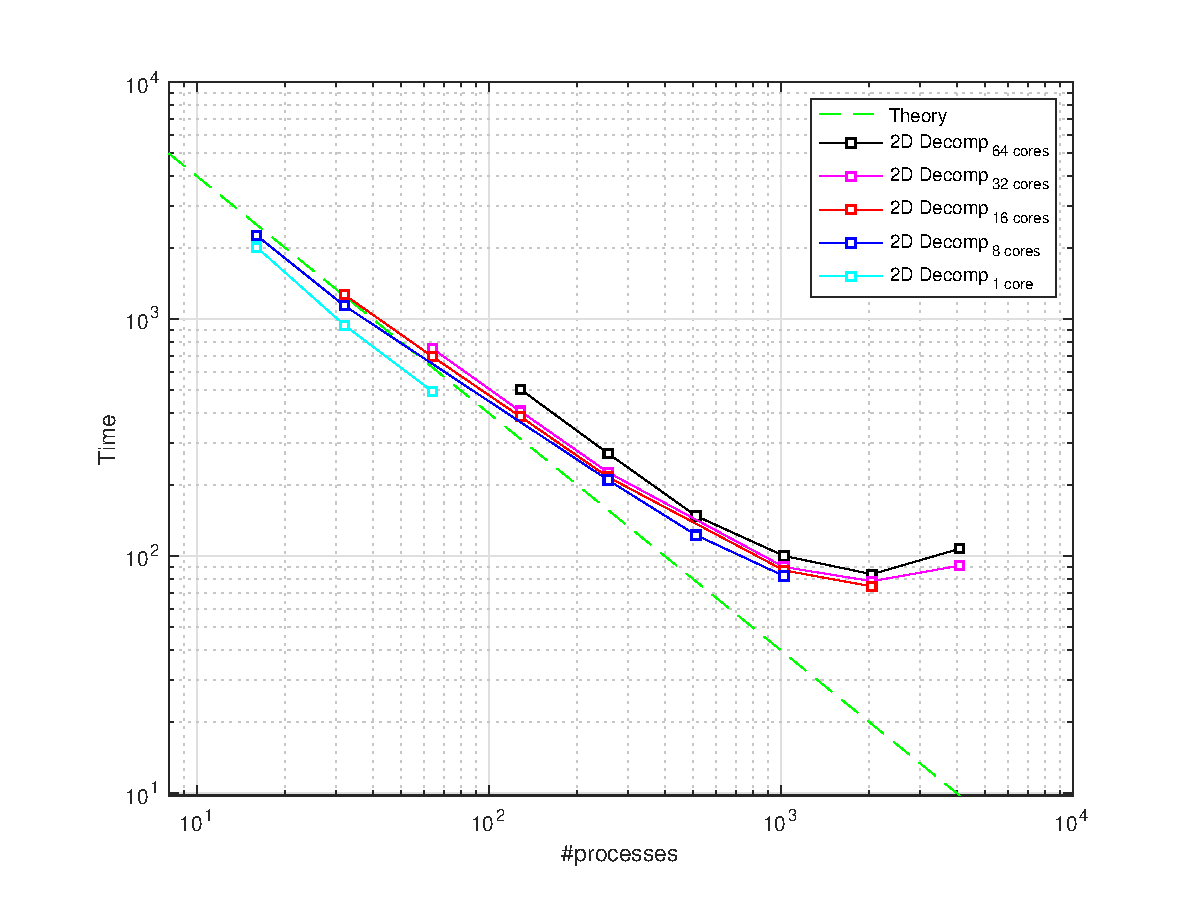
\includegraphics[scale=0.6]{grafici/5124}
\caption{Time scaling comparison for $512^3$ simulation}
\label{512:times}
\end{center}
\end{figure}

\begin{figure}
\begin{center}
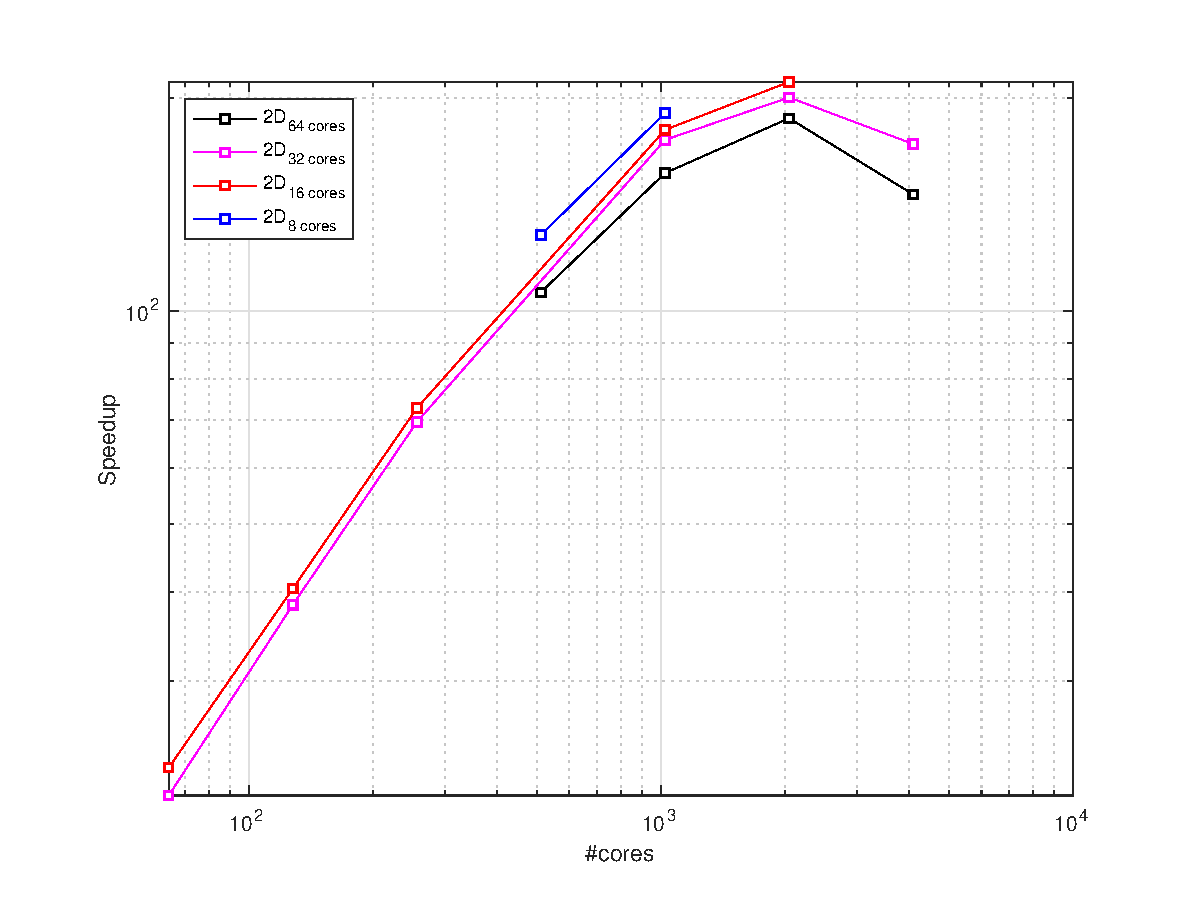
\includegraphics[scale=0.6]{grafici/5125}
\caption{Speedup factor comparison for $512^3$ simulation}
\label{512:perf}
\end{center}
\end{figure}

\begin{figure}
\begin{center}
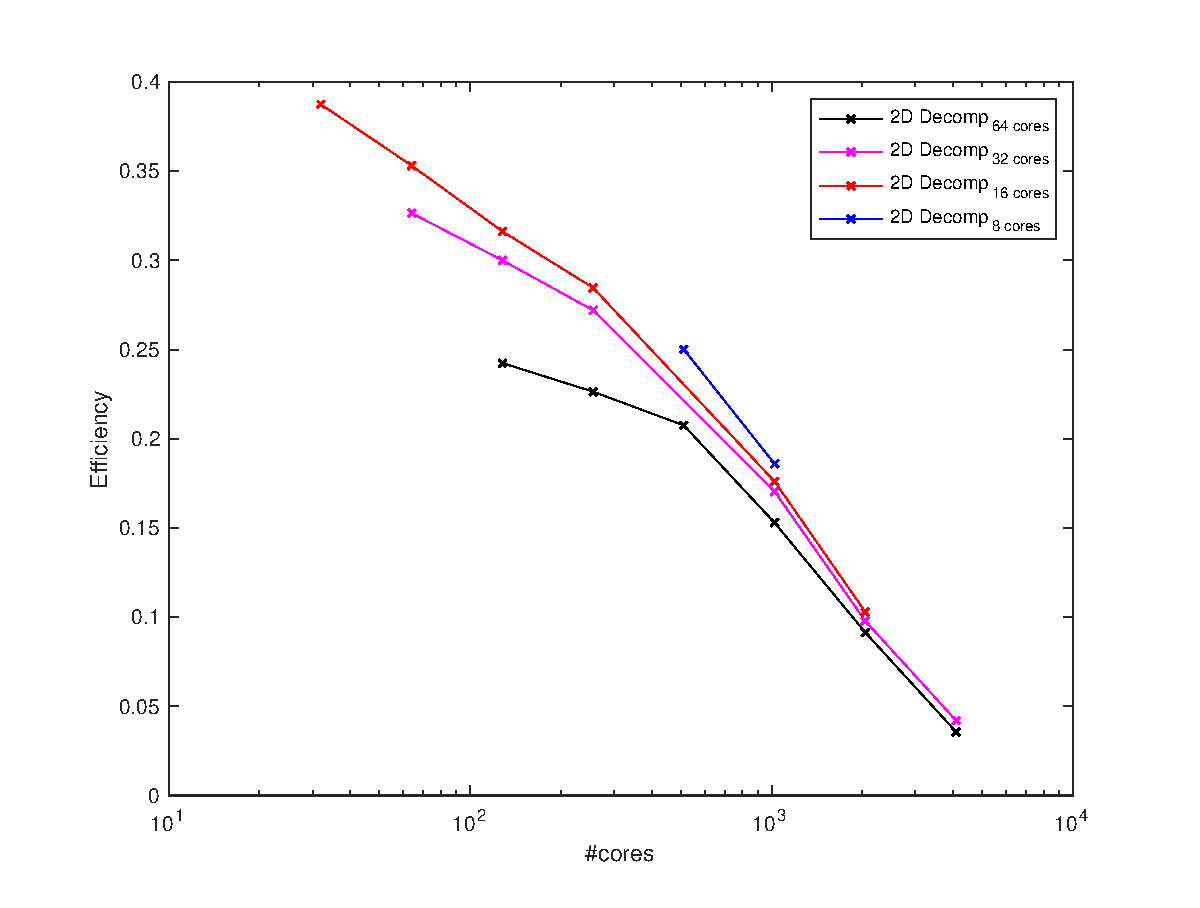
\includegraphics[scale=0.6]{grafici/5126}
\caption{Efficiency comparison for $512^3$ simulation}
\label{512:eff}
\end{center}
\end{figure}